%======================================================================
\subsection{BW-PDM-09 --- Plan: metric and inch, the product tree with drawings, and New Project (24 Oct 2026, approved 24 Oct)}\label{sec:pdm09-plan}
%======================================================================

You asked on 24 Oct for three things the vault does not do yet. This plan covers all three, because they share their
data: the units a project is drawn in, the tree of what a project is made of with each item's drawing, and a wizard
that creates that tree in one go. Your answers so far:
\begin{center}
\small
\begin{tabularx}{\linewidth}{@{}>{\raggedright\arraybackslash}p{3.2cm}X@{}}
\toprule
Feature & Your answer (24 Oct)\\
\midrule
A. Metric and inch & ``We will also need metric and imperial support.'' Chosen: \textbf{a default per vault (mm or inch)
  with an override per document}. New parts, drawing templates, title and tolerance blocks, sheet-metal gauges and
  lumber follow it.\\
B. Product tree with drawings & Top assembly $\rightarrow$ sub-assemblies $\rightarrow$ parts, each row with
  \code{P/N-REV}, state and its drawing (open, missing, out of date), like SolidWorks PDM or Onshape's structure view.\\
C. New Project wizard & Chosen: \textbf{structure and files}. Name the project, type or paste its structure with
  quantities; it numbers every item, writes the files (assemblies linking their children, empty drawings from the
  vault template), checks them in as WIP~01, and uses the units of~A.\\
\bottomrule
\end{tabularx}
\end{center}
It builds on the folder vault (\eref{PDM-04}), the per-revision BOM (\eref{PDM-06}, \S\ref{sec:pdm06-plan}), the drawing
standards (\eref{DRW-01}, \S\ref{sec:drw01-plan}) and the right panel's Vault tab (\eref{UIX-12},
\S\ref{sec:uix12-plan}).

%----------------------------------------------------------------------
\subsubsection*{1. What the spikes showed (24 Oct)}

Two scripts ran in \code{FreeCADCmd} 1.1.4 on a copy of your configuration, everything in a scratch folder
(\file{project-plan/spike\_units.py} and \file{spike\_project.py}). The second made a scratch vault with program
\code{DM} and inch drawing standards, then did by hand what the wizard would do for a small cart: seven items (two
assemblies, four parts, one COTS caster), six drawings, every file checked in as WIP~01.
\begin{center}
\small
\begin{tabularx}{\linewidth}{@{}>{\hsize=1.1\hsize}X>{\hsize=0.9\hsize}X@{}}
\toprule
Units: check & Result\\
\midrule
Per-document unit system in 1.1 & \code{Document.UnitSystem}, an enumeration of the 10 schemas, saved in
  \file{Document.xml} as an index (\code{3} = Imperial decimal), read back after reopening\\
What is stored & always mm: a 2\,in box saves \code{Length = 50.8}\\
Who switches the display & the GUI, when a document becomes active (\file{Gui/Application.cpp}), unless
  \code{IgnoreProjectSchema} is set; headless nothing switches\\
Decimals & \emph{one} global setting (\code{Units/Decimals}, default 2); no Python setter, and the per-document switch
  does not touch it\\
Imperial decimal, 2 decimals & $\tfrac18$\,in shows \code{0.13 in}, 0.001\,in shows \code{0.00 in}: too coarse\\
US customary (the other inch schema) & 0.5\,mm shows \code{19.69 thou}, 48\,in shows \code{1.33 yd}; a 36\,in
  dimension on a drawing reads \code{1.00 yd}: unusable for parts\\
Building US (feet--inches) & fractions to $\tfrac18$, 0.5\,mm shows \code{0}\\
Typed input & \code{1/4 in}, \code{1/4"}, \code{2' 3"} parse; \code{1 1/2 in} and \code{3/8in + 2mm} do not\\
TechDraw dimension text & follows the \emph{global} schema at recompute: \code{914.40 mm}, \code{36.00 in},
  \code{1.00 yd} or \code{3'} for the same edge; format \code{\%.2w}\\
\bottomrule
\end{tabularx}
\end{center}
\begin{center}
\small
\begin{tabularx}{\linewidth}{@{}>{\hsize=1.1\hsize}X>{\hsize=0.9\hsize}X@{}}
\toprule
New project: check & Result\\
\midrule
Numbers & 13 numbers from \code{JsonNumberSource.allocate}, one parent each; \emph{family} numbers (subs under the
  top's parent) collide, because the parent counters are per document type\\
Assembly linking part files, headless & works: save the assembly first, then one \code{App::Link} per instance;
  reopening the top loaded all 7 files, no broken link, \code{UnitSystem} kept\\
Assembly BOM of the result & quantities right (2, 3, 4, 4); each part also lists its \code{Body} (the walker of
  \eref{PDM-06} drops bodies)\\
Empty drawing per item (\code{new\_drawing} on a link to the model) & works, with ``Source shape is Null'' warnings
  while the part is empty; the drawing file's only XLink is its model, so \code{drawing\_of} can be read back\\
\quad its title block & company, units (\code{inch}), standard, projection and tolerances filled; \textbf{P/N blank and
  title ``Model''}: \code{part\_of} does not follow an \code{App::Link} to another file\\
Template switch (ANSI B $\rightarrow$ ISO A3) & setting \code{Template} \textbf{drops every filled field}; only the fill
  observer's merge (\code{\_ensure\_variant}) keeps them\\
Check-in of 13 files as WIP~01 & works; FreeCAD left an \file{.FCBak} beside each work file (the GUI turns backups off for
  vault files, the wizard must too)\\
Out of date, by recorded version & after a side-rail change: only the side rail's drawing is out of date (exact)\\
\code{release\_check.where\_used} of the side rail & lists the assemblies \emph{and} three drawings (they link a file
  that links it): the tree must keep drawings out of the structure\\
Drawing number with a suffix (PDM-07 Q4) & \code{\ldots-001-DWG} is read as revision \code{DWG} and stripped to the part's
  key; \code{\ldots-001.DWG} is refused by the parser\\
\bottomrule
\end{tabularx}
\end{center}

\paragraph{Four findings to act on.} (1) Inch needs three decimals while mm wants two, and FreeCAD has one global
setting: the document switch must set decimals too (a small \code{[BW]} change). (2) Only \emph{Imperial decimal} suits
inch parts; the vault must never offer US customary. (3) The drawing filler must follow a link into the model's file,
or a drawing kept in its own file (as the vault wants it) gets no P/N. (4) A drawing key with a suffix needs explicit
support in \file{numbering.py}; the form is \eref{PDM-07}'s to settle (Q4 there), and this plan only needs the
lookup \emph{drawing of P/N} to work.

%----------------------------------------------------------------------
\subsubsection*{2. A --- Metric and inch}

\paragraph{Theory: units are a view, not data.} Every length is stored in millimetres, so a value $v$ (mm) is shown in
unit $u$ with $d$ decimals as $\mathrm{round}(v/u, d)$, with $u = 1$ for mm and $u = 25.4$ for inch (exact by
definition since 1959). Converting loses nothing; only the \emph{display} rounds, with a worst-case error
\[
  e_{\max} = \tfrac12\, u\, 10^{-d}\ \text{mm}:
  \qquad
  \begin{array}{@{}l@{\quad}l@{}}
  \text{mm},\ d=2:\ 0.005\,\text{mm} & \text{in},\ d=2:\ 0.127\,\text{mm}\\
  \text{in},\ d=3:\ 0.0127\,\text{mm} & \text{in},\ d=4:\ 0.00127\,\text{mm}.
  \end{array}
\]
A machinist reads \code{.125} as $\tfrac18$; at $d=2$ the screen says \code{0.13}, an error of 0.127\,mm, as large as
a typical $\pm$.005\,in tolerance. So inch documents need $d \ge 3$, and $d = 4$ where ten-thousandths matter (bearing
fits). Fractions are a second display, $\mathrm{round}(v/u \cdot 2^k)/2^k$ with $k$ from \code{FracInch} (8 = $\tfrac18$),
useful for lumber and frames, wrong for machined parts. Typed values parse in the unit written (\code{1/4 in} is
6.35\,mm); a \emph{bare} number in an expression is mm whatever the schema, the one trap the per-document switch
cannot remove (risks).

\begin{figure}[!htbp]
\centering
\begin{tikzpicture}[>=Stealth,node distance=4mm and 7mm,
  b/.style={draw=bwblue!70,fill=bwblue!5,rounded corners=2pt,font=\scriptsize,align=center,minimum height=1.0cm,text width=2.5cm},
  g/.style={b,draw=bwgreen!80,fill=bwgreen!8},
  o/.style={b,draw=bworange!80,fill=bworange!8},
  t/.style={font=\tiny\color{bwgrey},align=center}]
\node[g] (v) {Vault default\\\texttt{units: mm | in}\\(Vault Settings, CSV)};
\node[b,right=of v] (d) {New document\\\texttt{UnitSystem} = Standard or Imperial decimal};
\node[o,right=of d] (a) {Document activated\\schema \emph{and} decimals switch\\(\code{[BW]})};
\node[b,right=of a] (s) {Shown: Properties, Parameters, Physical, sketches, dimensions};
\node[b,below=7mm of d] (dr) {New drawing\\sheet, tolerance block, format by unit};
\node[b,below=7mm of a] (sm) {Sheet-metal rules\\gauge label, $T$ in the unit};
\node[b,below=7mm of s] (fr) {Frame and lumber\\inch families, fractions};
\draw[->] (v) -- (d); \draw[->] (d) -- (a); \draw[->] (a) -- (s);
\draw[->] (v.south) |- (dr.west);
\draw[->] (a) -- (sm); \draw[->] (a.south east) -- (fr.north west);
\node[t,above=1mm of d] {override: the document's own setting};
\node[t,above=1mm of s] {stored: always mm};
\end{tikzpicture}
\caption{Where the unit choice comes from and what follows it. Green is the vault's setting, orange the one upstream
change.}
\label{fig:pdm09-units}
\end{figure}

\paragraph{Design.}
\begin{itemize}[nosep]
  \item \textbf{The vault default} is the \code{units} setting that \file{drawing\_standards.json} already has (DRW-01:
        \code{mm} or \code{in}, in Vault Settings and the CSV). It widens from ``what the title block says'' to ``what new
        documents use''. The Create Vault wizard asks it on its first page.
  \item \textbf{Two profiles, nothing else.} \code{mm} $\mapsto$ \emph{Standard (mm, kg, s, \textdegree)}, 2 decimals;
        \code{in} $\mapsto$ \emph{Imperial decimal (in, lb)}, 3 decimals (question~2). US customary, feet--inches and the
        rest stay available in FreeCAD's own menu but are never set by Vector Labs.
  \item \textbf{The override} is the document's own \code{UnitSystem}, set when Vector Labs creates a document (New Part,
        New Assembly, New Drawing, the wizard) from the vault or the project, and changed from the status bar's unit
        button as today. The status-bar readout gains ``inch'' or ``mm'' beside the vault name, and a document whose units
        differ from its vault's shows them in the Vault tab's header (the ``in'' badge in figure~\ref{fig:pdm09-tree}).
  \item \textbf{Decimals per unit.} \code{[BW]} in \file{Gui/Application.cpp}: when the active document switches the
        schema, decimals come from \code{Units/DecimalsMetric} (2) or \code{Units/DecimalsInch} (3) by the schema's
        length unit; the pack writes both and keeps \code{IgnoreProjectSchema} off. About 15 lines, an upstream candidate
        (upstream has one decimals setting for every schema).
  \item \textbf{Drawings.} The vault's drawing standards get a pair of profiles: sheet and tolerances for mm (ISO A3 or
        ANSI B with $\pm$0.5/0.25/0.1\,mm, as DRW-01) and for inch (ANSI B, X.X $\pm$.1, X.XX $\pm$.01, X.XXX $\pm$.005,
        angles $\pm$1\textdegree), surface finish in $\mu$m or $\mu$in (already done). A new drawing takes the profile of
        its \emph{model's} units; the dimension format is \code{\%.2w} for mm and \code{\%.3f} for inch (ASME: trailing
        zeros to the tolerance's places). TechDraw cannot drop the leading zero (\code{.250}, ASME inch); a \code{[BW]}
        option in \code{formatValueToSpec} is question~3. Changing a drawing's units later goes through the fill observer,
        which keeps filled and hand-typed fields (finding: a bare template switch loses them).
  \item \textbf{Sheet metal and lumber} (\S\ref{sec:mod06-plan}, \S\ref{sec:mod07-plan}). Rules stay in mm with the gauge
        as an alias (decided); in an inch document the rule list reads ``16\,ga (0.060\,in)'' and $T$, $R$ and the relief
        show in inch through the schema. Lumber keeps its nominal names and actual sizes; an inch document shows
        $1.5\times3.5$\,in, and its stock lengths and kerf (already per vault in feet and inches) need no change.
  \item \textbf{Mixed assemblies} need nothing: an inch part linked into a mm assembly is the same millimetres, shown
        in the assembly's units while the assembly is active.
\end{itemize}

%----------------------------------------------------------------------
\subsubsection*{3. B --- The product tree with drawings}

\begin{figure}[!htbp]
\centering
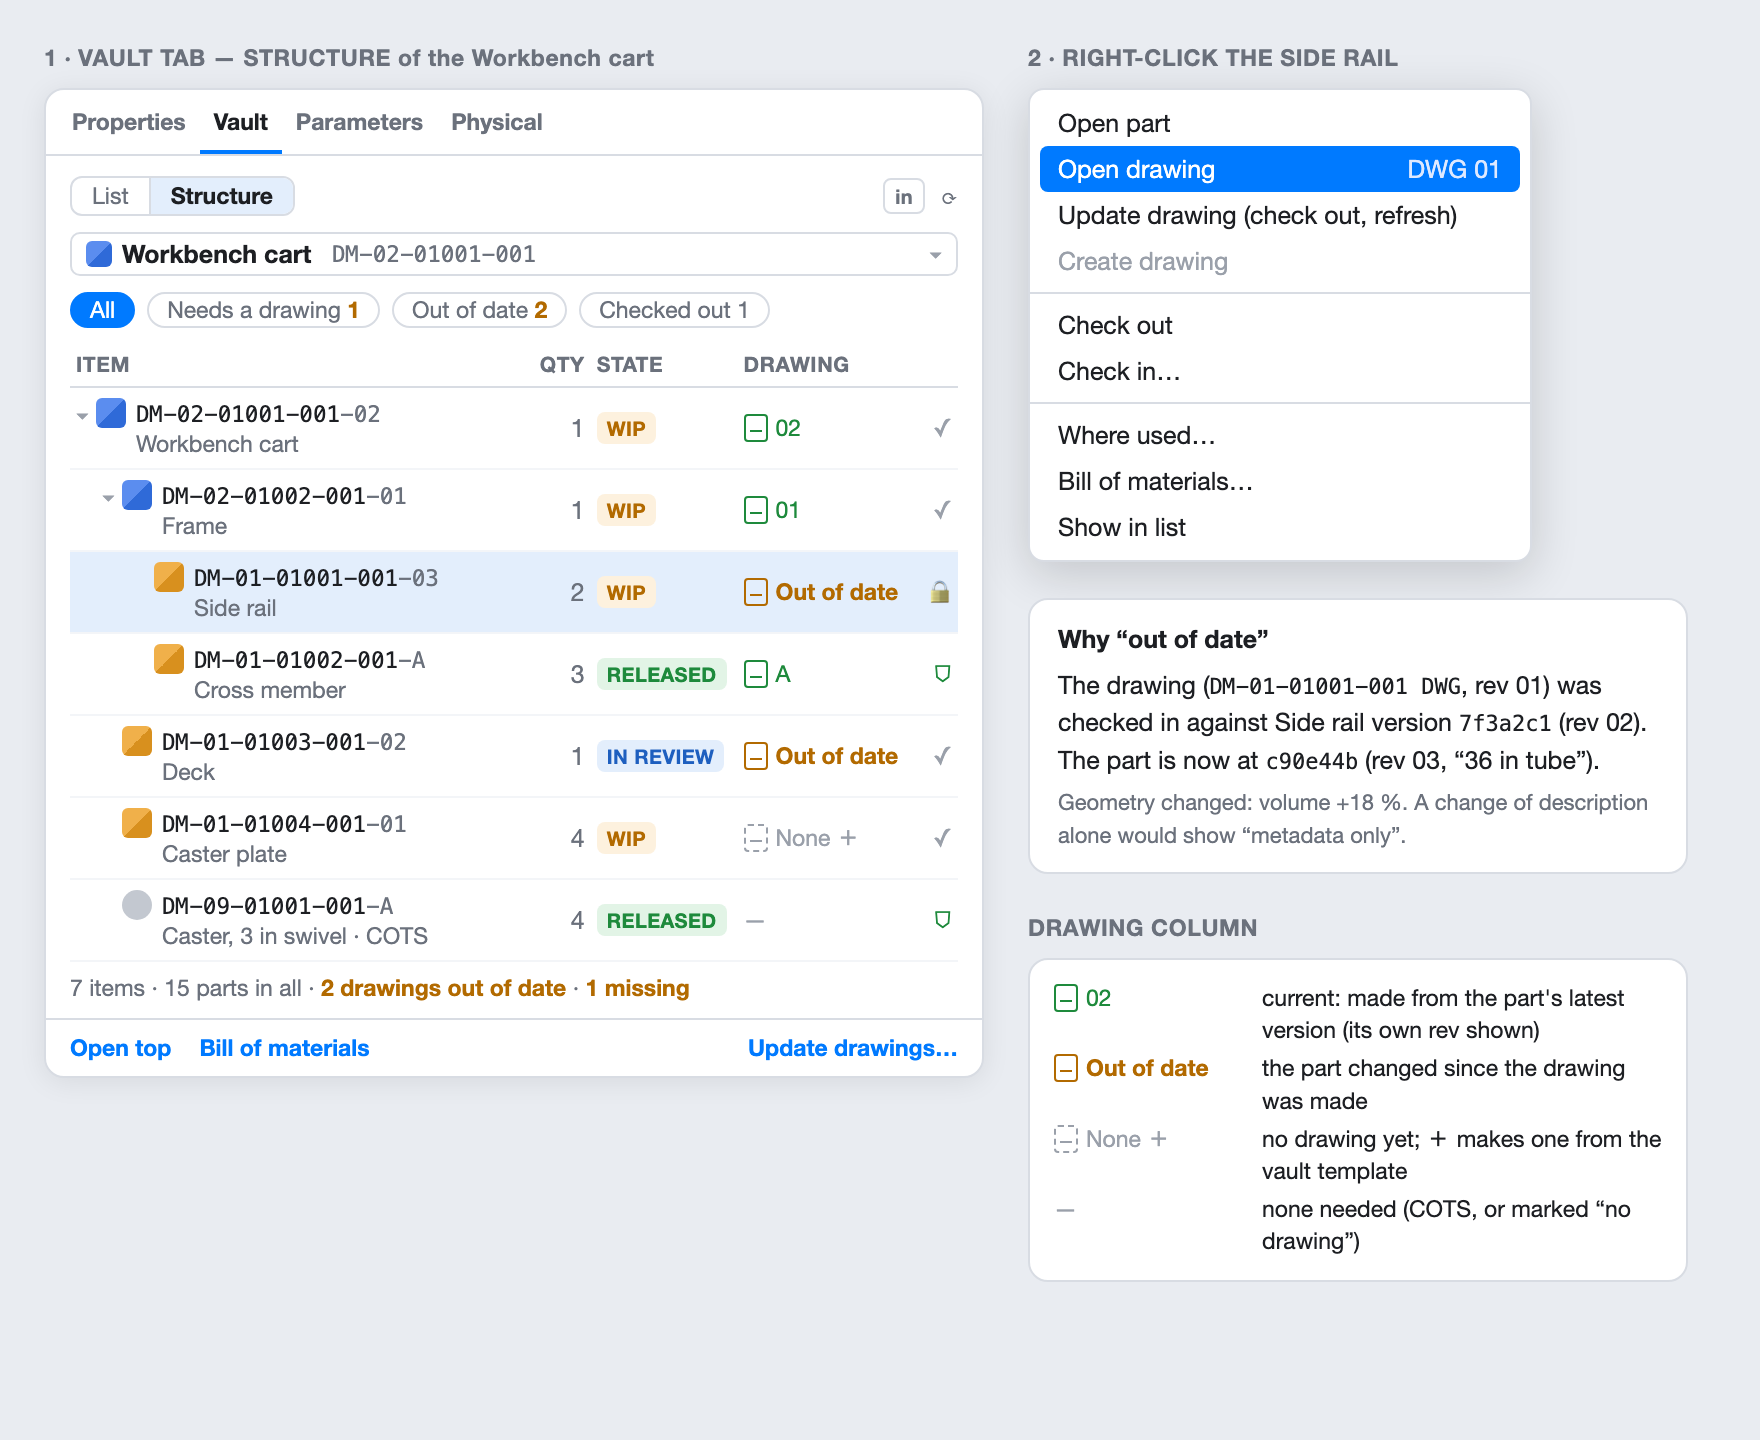
\includegraphics[width=\linewidth]{fig/pdm09_tree.png}
\caption{Mock: the Vault tab's \emph{Structure} view (left), the menu of a row, and why its drawing is out of date. The
list view of today's Vault card stays as \emph{List}. Light mode; the dark one follows the panel's tokens.}
\label{fig:pdm09-tree}
\end{figure}

\paragraph{Where it lives.} In the \textbf{Vault tab} of the right panel (\eref{UIX-12}; the tab is registered but still
a placeholder, and the floating Vault card retires into it). A segmented switch at its top chooses \emph{List} (the
card's list, unchanged) or \emph{Structure}. The root is picked at the top: a project (section~4), or any assembly; it
follows the Browser when an assembly is selected there. The footer offers \emph{Open top}, \emph{Bill of materials}
(\eref{PDM-06}) and \emph{Update drawings\ldots}, which checks out each out-of-date drawing, opens it, recomputes and
offers the check-in. A row's menu adds \emph{Open drawing}, \emph{Update drawing}, \emph{Create drawing}, \emph{Where
used\ldots} and \emph{Show in list}. Filter chips: \emph{Needs a drawing}, \emph{Out of date}, \emph{Checked out}; an
assembly row that hides a problem below it carries the count.

\paragraph{Where the rows come from.} The structure of revision $a$ is the per-revision BOM of \eref{PDM-06}
(lines to child items with quantity, resolved to child revisions). Until PDM-06 is built, and for versions checked in
before it, the rows come from the checked-in file's links (\code{release\_check.components\_of}), with the quantity
counted from the links, marked ``from links''. Drawings never become rows: an item's drawings are
\code{vault.drawings\_of(p)} (the \code{drawing\_of} link of \eref{PDM-02}), shown in the row's \emph{Drawing} cell. A
part file that still holds its own TechDraw page (DRW-01's \emph{New Drawing} puts the page there today) shows
``in model'' in that cell, so nothing looks missing that is not. The tree is rebuilt from the journal on every refresh,
$O(|R|+|E|)$ as in \S\ref{sec:pdm06-plan}, and drawn lazily, one level at a time.

\paragraph{Theory: when is a drawing out of date?} A drawing $D$ of model $m$ is right when it was last made from the
model as it is now. A time comparison (``$D$ checked in before $m$'') is not that: a drawing checked in later only to fix
a note was still made from whatever model its work folder held, and a drawing made from an older model fetched with
\emph{Get Revision} would look current. So the check-in records what the drawing was made from. Let $v(x)$ be the
latest version (SHA-256) of item $x$ and $C(D)$ the closure of files $D$ links to (for a part drawing, the part; for an
assembly drawing, the assembly and everything under it). When $D$ is checked in, its event records
\[
  r_D = \{\,x \mapsto b(x) : x \in C(D)\,\},
\]
where $b(x)$ is the base version of $x$'s work copy (\code{state.json}), exactly the file FreeCAD had open. Then
\[
  \mathrm{state}(D) =
  \begin{cases}
    \text{missing} & \text{if } m \text{ needs a drawing and } \mathrm{drawings}(m) = \varnothing,\\
    \text{out of date} & \text{if } \exists\, x \in C(D):\ r_D(x) \ne v(x),\\
    \text{current} & \text{otherwise.}
  \end{cases}
\]
For a released drawing, $v$ is the \emph{released} version of each $x$. Not every new version matters: a description
edit changes the file's hash but not one line on the sheet (the fill observer refreshes the title block by itself).
So each part check-in also records a geometry fingerprint $g$ (volume, area, centre of mass and bounding box, rounded
to $10^{-6}$ relative, the same mass properties \eref{PDM-08} uses to check a migration), and a drawing whose $r_D(x)$
differs only where $g$ is equal shows ``metadata only'' in grey instead of orange. Drawings checked in before this
epic have no $r_D$; they fall back to the time comparison and say so.

\begin{figure}[!htbp]
\centering
\begin{tikzpicture}[>=Stealth,x=1.6cm,y=-1.0cm,
  v/.style={circle,draw=bwblue,fill=white,inner sep=1.4pt,font=\tiny,minimum size=6mm},
  d/.style={circle,draw=bworange,fill=white,inner sep=1.4pt,font=\tiny,minimum size=6mm},
  t/.style={font=\scriptsize,anchor=east},
  n/.style={font=\tiny\color{bwgrey},align=center}]
\node[t] at (-0.3,0) {Side rail (part)};
\node[t] at (-0.3,1.6) {Its drawing};
\draw[black!25] (-0.2,0) -- (6.2,0); \draw[black!25] (-0.2,1.6) -- (6.2,1.6);
\node[v] (p1) at (0.3,0) {01}; \node[v] (p2) at (2.2,0) {02}; \node[v] (p3) at (3.8,0) {02$'$};
\node[d] (d1) at (1.1,1.6) {01}; \node[d] (d2) at (5.3,1.6) {01$'$};
\draw[->,bworange] (d1) -- node[n,left=1pt,pos=0.4] {$r_D$} (p1);
\draw[->,bworange] (d2.north west) .. controls (3.2,1.0) and (1.2,0.9) .. node[n,below=1pt,pos=0.5] {$r_D = 01$} (p1.south east);
\draw[->,black!35,dashed] (d2.north) -- node[n,right=2pt,pos=0.45,text width=2.6cm,align=left] {had it been made from 02: ``metadata only''} (p2.south east);
\node[n] at (0.3,-0.6) {created}; \node[n] at (2.2,-0.65) {geometry\\changed}; \node[n] at (3.8,-0.65) {description\\only};
\node[n] at (1.1,2.25) {made from 01};
\node[n] at (5.3,2.35) {note fixed, checked in last;\\its work copy still held part 01};
\end{tikzpicture}
\caption{Why the drawing records the version it was made from. Its second check-in comes after every part version, so a
time rule calls it current; but it was made from part 01, and the geometry changed in 02, so it is out of date. Had it
been made from 02, only the description would differ (same fingerprint): ``metadata only''.}
\label{fig:pdm09-outofdate}
\end{figure}

\paragraph{Journal.} The check-in event gains an optional \code{made\_from} map (P/N $\rightarrow$ SHA-256) and, for
parts, \code{fingerprint}; older journals replay unchanged. Both come from the FreeCAD side at check-in (it has the
document open and the workspace's bases), so \file{pdm\_folder.py} stays free of FreeCAD. The release checklist
(\eref{PDM-05}) gains a line ``drawing current'' that blocks a release of a part whose drawing is out of date
(question~6).

%----------------------------------------------------------------------
\subsubsection*{4. C --- New Project}

\paragraph{What a project is.} The vault has \emph{programs} (the numbering prefix: \code{LE}, \code{BW}) and items;
work files live flat in \file{work/<user>/<P/N>.FCStd} and are named by number, so a folder per project would fight the
vault's layout. Four options:
\begin{center}
\small
\begin{tabularx}{\linewidth}{@{}>{\raggedright\arraybackslash}p{3.1cm}XX@{}}
\toprule
A project is \ldots & For & Against\\
\midrule
a program code & exists today; numbers show it & a program is a product line with many projects (LE has the pedestal,
  the arm, \ldots); programs are retired, never deleted\\
a folder & familiar & the vault has no folders: files are named by P/N, the work folder is flat\\
a record in vault settings & edited with the other settings & settings are one file one writer at a time, and they
  have no history\\
\textbf{a journal record} (proposed) & replays like every item; has history; one writer per file, sync-safe & a new
  operation in the contract\\
\bottomrule
\end{tabularx}
\end{center}
Proposed: an operation \code{create\_project} with a code, name, program, top assembly P/N, units and drawing profile,
and \code{update\_project} to rename or close it. The project's \emph{structure} is never stored twice: it is the top
assembly's BOM, so it changes when the assembly does. A project is what the Structure view's picker lists, what the
Start page shows as recent work, and the units default for new documents in it (sitting between the vault's and the
document's).

\begin{figure}[!htbp]
\centering
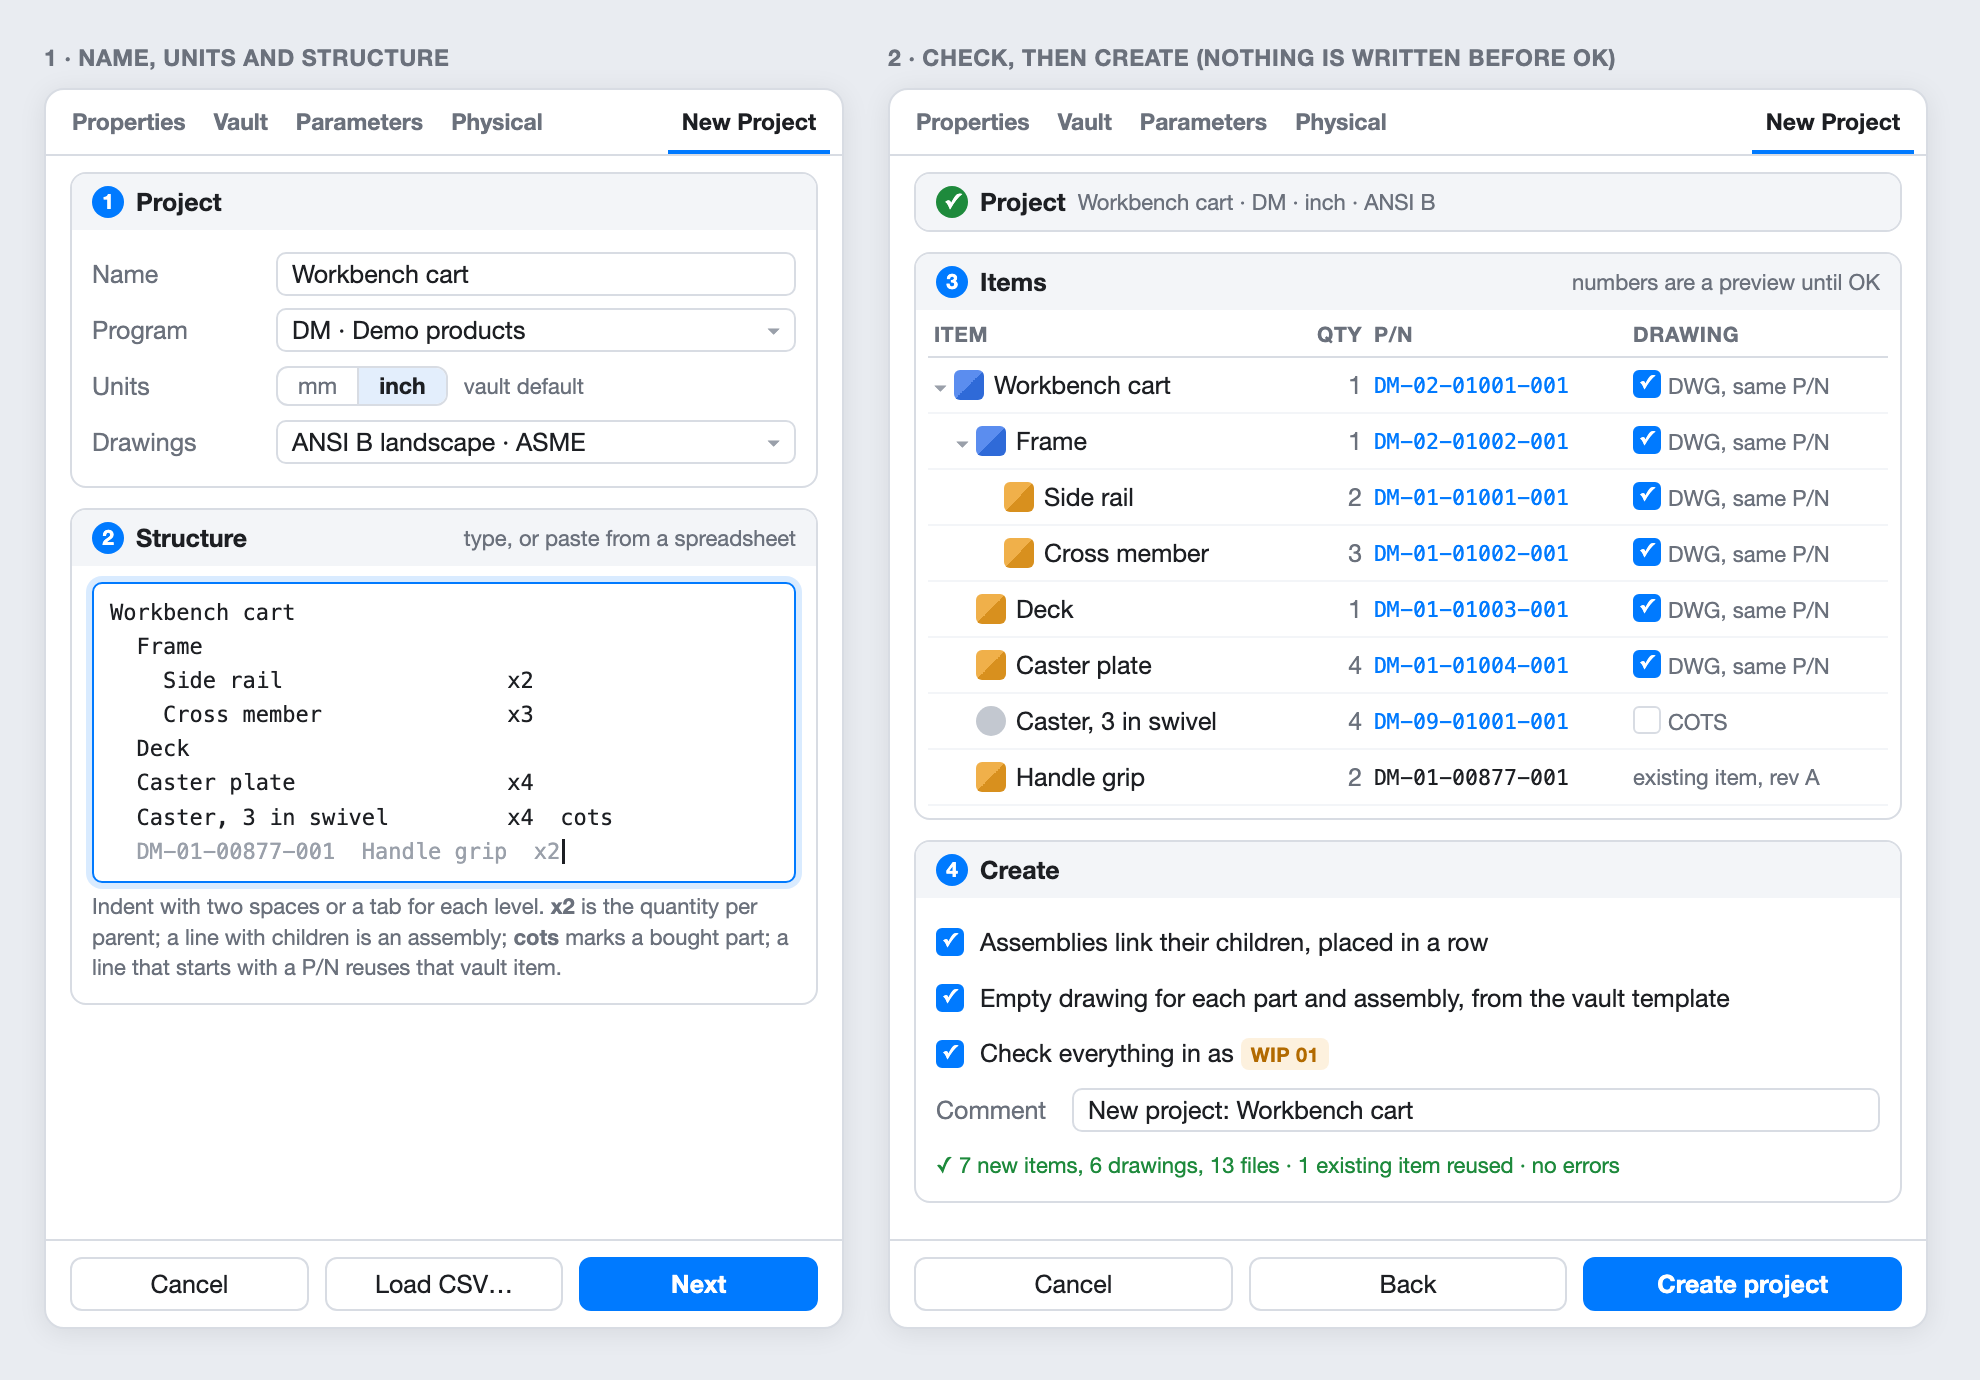
\includegraphics[width=\linewidth]{fig/pdm09_wizard.png}
\caption{Mock: \emph{New Project} as a task panel, the right panel's command tab, like Create Vault. Left: name,
program, units and drawing profile, and the structure typed as indented lines. Right: the preview with numbers, each
item's drawing, and what will be created. Nothing is reserved or written before \emph{Create project}. Drawings carry their
part's number, as decided for \eref{PDM-07} (Q4).}
\label{fig:pdm09-wizard}
\end{figure}

\paragraph{The structure, as typed.} One line per item; two spaces or a tab per level; \code{x}$n$ is the quantity per
parent (default 1); a line with children is an assembly; \code{cots} marks a bought part (no drawing); a line that
starts with a P/N reuses that vault item. A paste from a spreadsheet with columns \emph{level, name, qty, type} is read
the same way, and \emph{Load CSV\ldots} takes the file. The text maps to a rooted tree $T$; the same name in two places
is the same item (a bolt in two sub-assemblies), so $T$ is a DAG, and indentation cannot make a cycle. The preview shows
$Q_t$ (the roll-up of \S\ref{sec:pdm06-plan}) as ``15 parts in all'', so a mistyped quantity shows before anything is
made.

\paragraph{What Create does.} In this order, so that a failure leaves nothing half-made in the vault:
\begin{enumerate}[nosep]
  \item \textbf{Check} (preview, nothing written): names, quantities, reused P/Ns exist and are not obsolete, program
        and document types not retired.
  \item \textbf{Write files in staging} (\file{<vault>/.import}, as the import does), children first: a part is an
        \code{App::Part} with a body and the vault's part properties (\file{partprops.py}); an assembly is an
        \code{Assembly::AssemblyObject} saved \emph{before} its links are made (spike), with one \code{App::Link} per
        instance placed in a row, the first child grounded; a drawing is its own file with a hidden link to its model and
        a page from the vault's template for the project's units, with front, top and right views that fill in once the
        part has a shape. Every document gets the project's \code{UnitSystem}; backups off.
  \item \textbf{Verify}: reopen the top from staging; every link resolves and every count matches $T$.
  \item \textbf{Allocate and commit}: reserve the numbers (flat, one parent each; family numbers collide, see the spike),
        rename the staged files to \file{<P/N>.FCStd} and rewrite their links (\code{rewrite\_links}, as the import
        does), write the P/N into each file, then \code{create\_item} for every item and drawing,
        \code{create\_project}, and one check-in per file with the comment, all WIP~01. A file that fails here leaves its
        number unused and is listed, like \code{run\_import}.
  \item \textbf{Open} the top assembly and show its Structure.
\end{enumerate}
The engine is a new FreeCAD-free module \file{bruceworx/project\_setup.py} (parse, check, plan numbers, the order of work)
with a small FreeCAD side for steps 2--3 that can run headless, so the same thing is \code{bw-hooks project new
--structure cart.txt} from the command line. Entry points: \emph{File $\rightarrow$ New Project\ldots}, the Start page,
Cmd-K, and the Structure view's empty state.

%----------------------------------------------------------------------
\subsubsection*{5. Build order and effort}

\begin{center}
\small
\begin{tabularx}{\linewidth}{@{}lXl@{}}
\toprule
\# & Step & Effort\\
\midrule
1 & Units: vault default used for new documents; the two profiles; \code{[BW]} decimals per unit; pack entries;
  status-bar readout; tests & 1.5\,d\\
2 & Drawings by unit: mm and inch profiles in the drawing standards (CSV, Vault Settings), dimension format; fix
  \code{part\_of} to follow links; template change through the observer & 1.5\,d\\
3 & Sheet-metal and lumber labels in inch documents (with \eref{MOD-06} and \eref{MOD-07}, which are building) & 0.5\,d\\
4 & Journal: \code{made\_from} and \code{fingerprint} on check-in, \code{create\_project}; contract tests; OpenAPI & 1\,d\\
5 & Structure view: tree model (BOM, or links until \eref{PDM-06}), drawing states, filters, menu, \emph{Update drawings}
  in the Vault tab & 2.5\,d\\
6 & \file{project\_setup.py}: parser (text, paste, CSV), check, plan; FreeCAD-free tests & 1\,d\\
7 & File writer (staging, verify, commit) and the New Project task panel & 2.5\,d\\
8 & Release checklist line ``drawing current''; acceptance on a scratch vault, then a real one; write-up & 1\,d\\
\midrule
 & Total & 11.5\,d\\
\bottomrule
\end{tabularx}
\end{center}
Steps 1--3 stand alone and help the drawings now being built; step~5 needs the Vault tab of \eref{UIX-12} and is exact
once \eref{PDM-06} keeps BOMs per revision. \emph{Acceptance:} a project typed as six lines becomes numbered part,
assembly and drawing files checked in as WIP~01 in inch; changing one part marks exactly its drawing (and the drawings
of the assemblies above it) out of date in the Structure view.

\paragraph{Risks.} \emph{Bare numbers in expressions} are millimetres in an inch document (\code{=2} is 2\,mm); the
Parameters tab will show each expression's unit, and the sketcher's typed values already carry the schema's unit
\verify. \emph{Global schema}: two documents open side by side show the active one's units, so a mm assembly with an
inch part open in another tab switches as you click; this is FreeCAD's behaviour and stays. \emph{Upstream change}:
the decimals rule touches \file{Gui/Application.cpp} (one \code{[BW]} block). \emph{Empty drawings} warn in the report
view until their part has a shape; the warning is harmless but noisy, so the views may instead be added on first
open (question~8). \emph{Number gaps}: a failed commit leaves numbers unused, as an import does.

%----------------------------------------------------------------------
\paragraph{Your answers (24 Oct).} Recommendations for 1--5, 7, 9 and 11. Three changes:
\textbf{6} an out-of-date drawing \emph{warns} at release (a checklist line, not a block);
\textbf{8} the wizard creates \emph{blank} drawings (sheet and filled title block), with an option to insert the views
(\emph{Insert views} on the drawing, and a wizard tick box, off by default);
\textbf{10} a name typed twice is marked with a \emph{duplicate} bubble in the preview: you keep it as one item used
twice, or rename a line to make two items.

\subsubsection*{Questions before PDM-09 starts}

\begin{enumerate}
  \item \textbf{Three layers of units.} Vault default, project, document --- or only vault and document as you said?\\
        \emph{Recommendation:} keep your two, and let a project store the units it was created with, so its new parts
        follow it in a mm vault with one inch project. It costs one field.
  \item \textbf{Inch decimals.} 3 decimals (\code{.125}) or 4 (\code{.1250}) on screen?\\
        \emph{Recommendation:} 3 on screen and on drawings; 4 can be set per dimension where a fit needs it.
  \item \textbf{ASME leading zero.} ASME inch drawings write \code{.250}; TechDraw writes \code{0.250}. Add a \code{[BW]}
        option to drop it?\\
        \emph{Recommendation:} yes, on by default for inch drawings under ASME; it is a few lines and an upstream
        candidate.
  \item \textbf{Inch sheets.} Inch drawings on ANSI sheets only, and mm on ISO or ANSI as the vault says?\\
        \emph{Recommendation:} yes: inch $\rightarrow$ ANSI B with ASME; mm keeps DRW-01's choice (ANSI with mm).
  \item \textbf{Where the tree lives.} The Vault tab's \emph{Structure} view, or a separate window?\\
        \emph{Recommendation:} the Vault tab (figure~\ref{fig:pdm09-tree}), with \emph{Open in window} for a big tree
        later if the panel is too narrow.
  \item \textbf{Out-of-date drawings and release.} Block a release when a drawing is out of date, or warn?\\
        \emph{Recommendation:} block, with ``metadata only'' allowed; waivable with a note, like the other checklist
        lines.
  \item \textbf{What a project is.} A journal record naming its top assembly (section~4)?\\
        \emph{Recommendation:} yes; programs stay the numbering prefix, folders stay out of the vault.
  \item \textbf{Empty drawings.} Create each drawing with its three views (filling in when the part has a shape), or
        only the sheet and title block, views added on first open?\\
        \emph{Recommendation:} with views; the warnings are silenced for empty sources.
  \item \textbf{Assembly drawings.} Is an assembly's drawing out of date when \emph{any} part below it changes geometry,
        or only when its own file changes?\\
        \emph{Recommendation:} any part below it (the closure $C(D)$), since its views show them; the chip says which.
  \item \textbf{Same name, same item.} When a name appears twice in a typed structure, is it one item used twice?\\
        \emph{Recommendation:} yes, and the preview marks it ``used in 2 places''; rename a line to make two items.
  \item \textbf{Drawing numbers.} The wizard needs the drawing key of \eref{PDM-07} Q4 (a drawing carries its part's
        number). The spike shows \code{-DWG} is read as a revision. Settle the form there first?\\
        \emph{Recommendation:} yes; until it is built the wizard numbers drawings with the drawing document type
        (\code{03}), as the vault does today.
\end{enumerate}

%----------------------------------------------------------------------
\subsubsection*{Built, 26 Oct: steps 1--3 (A --- metric and inch)}

Built in three commits by the units agent while the project agent built steps 4--7; the epic stays
\emph{In progress} until 4--8 land. Where you had not answered a question, the recommendation was taken (1--5,
7, 9, 11) and is marked below.

\paragraph{Step 1, units (\code{d5ca3eb}).} New module \file{src/Mod/BruceWorx/bruceworx\_units.py}: the two
profiles (\code{mm} $\mapsto$ schema~0 \emph{Standard}, 2 decimals; \code{in} $\mapsto$ schema~3 \emph{Imperial
decimal}, 3 decimals, question~2 as recommended), \code{document\_units}, \code{vault\_units},
\code{default\_units} and \code{apply\_units(doc, units)}, also reachable as
\code{bruceworx\_defaults.apply\_units} for New Project; a project's units go through
\code{bruceworx\_units.DEFAULT\_HOOKS} (question~1: your two layers, plus the one field a project stores, as
recommended). New Part in Vault and the import writer (\code{freecad\_io.write\_part\_number(\ldots, units=)})
set the vault's units; in the GUI a document observer gives \emph{every} document created while a vault is
open the default, so the Start page's New Part / New Assembly (\code{Std\_New}) and the wizard's files get it
without a call. The \code{[BW]} block in \file{Gui/Application.cpp} (13 lines): on the schema switch, decimals
come from \code{Units/DecimalsMetric} or \code{Units/DecimalsInch} by the schema's length unit (\code{in} and
\code{ft} count as inch); without the keys stock behaviour is unchanged. The pack writes 2 and 3, keeps
\code{IgnoreProjectSchema} off and turns on \code{Mod/TechDraw/Dimensions/DropLeadingZeroInch}. The status bar
reads ``Vault Vector~·~mm''; the right panel's Vault tab reads ``Vault~·~in'' when the active document's units
differ from the vault's (\code{bruceworx\_rightpanel.BADGES}, the only change to that module: the tab body is
step~5's). The Create Vault page asks the units under Folder (step~3's commit).

\paragraph{Step 2, drawings by unit (\code{8050507}).} The drawing standards gain an inch profile beside
DRW-01's: \code{in\_default\_sheet} (ANSI~B), \code{in\_tol\_1\_place} .1, \code{in\_tol\_2\_place} .01,
\code{in\_tol\_3\_place} .005, \code{in\_tol\_angle} 1\textdegree, in the JSON (format version~2), the vault
CSV's \code{standard} rows and the Vault Settings box (``Sheet (mm)'', ``Sheet (inch)'', two tolerance
columns, a preview of both blocks). \code{drawing\_standards.profile(standards, units)} is the view a drawing
uses: inch drawings are ASME on ANSI sheets with decimal tolerances written \code{.005} (question~4 as
recommended; an ISO GPS vault's inch drawings cite ASME Y14.5-2018, and the ISO 2768 mode becomes decimal
places for them). A version-1 file whose units were \code{in} had typed its tolerances in inches: they move to
the inch profile when the file is read, and the mm profile gets its defaults back. A new drawing takes the
profile of its \emph{model's} document units: sheet, title block and the dimension format, \code{\%.3f} and
\code{\%+.3f} on inch drawings, \code{\%.2w} on mm ones; a format the user typed is left alone, and the fill
observer refills a model's drawings when its \code{UnitSystem} changes (a new \code{slotChangedDocument}).
\code{part\_of} follows an \code{App::Link} into the model's file, so a drawing kept in its own file gets the
model's P/N, title and units; \code{new\_drawing(part, doc=other)} makes such a drawing through a link (both
files must be saved first, the spike's rule). \code{set\_sheet(page, sheet)} changes the sheet through the fill
path, so filled and typed fields survive. The leading zero (question~3 as recommended): \code{[BW]}
\code{DimensionFormatter::dropLeadingZero} in TechDraw drops it from a length (never an angle) while an inch
schema is active and the preference is on, so \code{.250} and \code{±.005}.

\paragraph{Step 3, sheet metal and lumber (\code{3d7ef8c}).} Rules stay in millimetres with the gauge alias; in
an inch document the rule list reads ``16~ga (0.060~in)'': inch lengths keep three places as a shop drawing
writes them (they had four, \code{0.0598~in}), mm labels are unchanged; $T$, $R$ and the relief in the picker
already followed the document's units (MOD-06). Lumber: \eref{MOD-07} is not built, so there is nothing to
show in inch yet; its plan already keeps nominal names with actual sizes, and this step's rule
(\code{bruceworx\_units.document\_units}) is what it will read.

\paragraph{Tests.} Headless: \code{TestBruceWorxUnits} (profiles, every FreeCAD schema mapped, apply and
reopen, vault default and project hook, New Part in an inch vault, import writer),
\code{TestBruceWorxDrawing} (inch model, drawing in its own file, sheet change, units change), the standards'
stdlib tests (profile view, migration, formats, CSV rows), \file{test\_sheetmetal\_rules\_units.py}; DRW-01,
the vault wizard and sheet-metal suites still pass (60 FreeCAD tests, 509 stdlib). GUI: the decimals switch
(activating an inch document shows \code{0.250~in}, a mm one \code{6.35~mm}; \code{apply\_units} on the active
document switches at once) and the acceptance: a scratch vault created with \code{units=in}: New Part in Vault
opens in Imperial decimal with three decimals, its drawing is ANSI~B with the inch tolerance block and ASME
note, and a dimension of a quarter-inch cube is drawn as \code{.250} (read back from the page's exported SVG);
the same in a mm vault gives \code{6.35~mm}, ``X.X ±0.5'' and \code{6.35}, and the inch document under the mm
vault wears the ``in'' badge. The pack's stdlib tests cover the new entries.

\paragraph{Decided while building.}
\begin{itemize}[nosep]
  \item \textbf{Every new document, not only four commands.} The observer applies the vault's (or project's)
        units to any document created while a vault is open. Files being opened pass through it too and are
        harmless: their own \code{UnitSystem} is restored a moment later (a pre-1.0 file without one keeps
        the vault's, which is what you would want). Headless paths call \code{apply\_units} themselves.
  \item \textbf{Import sets the vault's units} on the imported file. Units are a view, so nothing in the
        file changes but how it is shown; a file deliberately kept in the other units can be switched back
        from the status bar.
  \item \textbf{The leading zero is a TechDraw preference qualified by the active schema}, not a per-drawing
        setting: it needs no new property, and inch drawings in a Vector Labs vault are ASME by question~4.
        An ISO GPS vault's inch drawings drop it too; the preference can be turned off.
  \item \textbf{The sheet stays when a model's units change}: the title block, tolerance block and dimension
        formats follow at once, the sheet (ANSI~B or ISO~A3) is chosen at creation and changed with
        \code{set\_sheet}, which keeps every field. Swapping the sheet by itself would move the views.
  \item \textbf{Inch-family schemas count as inch.} US customary, Building US and Civil documents are shown
        as ``in'' by the badge and the drawing profile, though Vector Labs never sets them.
  \item \textbf{Decimals keys only when present.} Stock FreeCAD without the pack is unchanged. While the keys
        exist they win over Preferences $\rightarrow$ General $\rightarrow$ Units ``Number of decimals'' at the
        next document switch (question below).
\end{itemize}

\paragraph{Questions after steps 1--3.}
\begin{enumerate}[nosep]
  \item Should Preferences $\rightarrow$ Units ``Number of decimals'' edit the \emph{mm} value
        (\code{DecimalsMetric}) so the two never disagree, and should the BruceWorx preference page show
        both? \emph{Recommendation:} yes, two spin boxes on the BruceWorx page (``Decimals: mm 2, inch 3'').
  \item Should a model's units change also swap its drawing's sheet (ANSI~B $\leftrightarrow$ ISO~A3) when
        the two profiles name different sheets? \emph{Recommendation:} no; offer \emph{Change sheet\ldots} on
        the drawing (it is one call) and leave the views where they are.
  \item Import: keep ``imported files take the vault's units'', or only files that still have FreeCAD's
        default? \emph{Recommendation:} keep it; the vault reads as one.
\end{enumerate}

%----------------------------------------------------------------------
\subsubsection*{Built, 26 Oct: steps 4--8 (B --- the product tree, C --- New Project)}

Built by the second PDM-09 agent alongside steps 1--3, in three commits (\code{9125bd3} the journal,
\code{2eba35e} the FreeCAD-free engine, \code{3a61662} the window), on the plan's recommendations and your three
changes of 24 Oct. All of steps 4--8 passed the plan's acceptance, first on a scratch inch vault, then on a copy of
Vector (never the real one).

\paragraph{Step 4 --- the journal.} \file{pdm.py} gained the \emph{project} record (\code{create\_project}: code,
name, program, top assembly, units \code{mm}|\code{in}, drawing profile; \code{update\_project}: rename, re-point,
change units, close and reopen) with its rules: a unique code, a name and a program required, the top an assembly
that is not obsolete. \file{pdm\_folder.py} replays both, and a check-in may carry \code{made\_from} (a drawing:
P/N $\rightarrow$ the SHA-256 of the version its work copy held, over the closure $C(D)$ of the files it links) and
\code{fingerprint} (a part: volume, area, centre of mass, bounding box and solid count, each to 7 significant
digits, about $10^{-6}$ relative), both written only when given, so every journal from before reads exactly as it
did. The workspace computes \code{made\_from} from its \file{state.json} bases; \file{docs/pdm-openapi.yaml} is
0.4.0-draft (\code{/projects}, \code{PATCH /projects/\{code\}}, the two check-in fields, a \code{Fingerprint}
schema); the contract table has rows P1, P2 and a check-in-extras test. The dashboard's \emph{Projects} section
lists the recorded projects once a vault has any (top assemblies stand in until then, as PDM-10 said).
\textbf{Every Keystone copy must know \code{create\_project}, \code{update\_project} and the two check-in fields
before the real vault uses them}: an older Keystone would list those journal lines as problems, as the 25 Oct
record says for Mark as COTS and configuration numbers.

\paragraph{Theory as code.} \file{bruceworx/product\_tree.py} (FreeCAD-free, 15 tests) is the plan's
section~3: \code{drawing\_state} compares $r_D$ with $v(x)$ over $C(D)$ (the released version of each $x$ for a
released drawing, else the latest), calls a change \emph{metadata} when the two versions' fingerprints are equal
and \emph{geometry} otherwise, and reports out of date / metadata only / current with the list of what changed;
a drawing without $r_D$ falls back to the time comparison and says so (\code{basis} \code{"time"}). The Drawing
cell of an item adds \emph{missing}, \emph{no file yet} (a drawing item without a version), \emph{in model} (the
part's own file holds a TechDraw page: read from the stored object, cached by SHA-256) and \emph{none needed}
(bought parts). \code{Tree} gives the rows one level at a time from \file{vault\_trees.structure} (the recorded
BOM, else the file's links, marked), the chip counts of everything strictly below an assembly, the flat roll-up
$Q_t$ for the List view, and the out-of-date drawings under a root for \emph{Update drawings}.

\begin{figure}[!htbp]
\centering
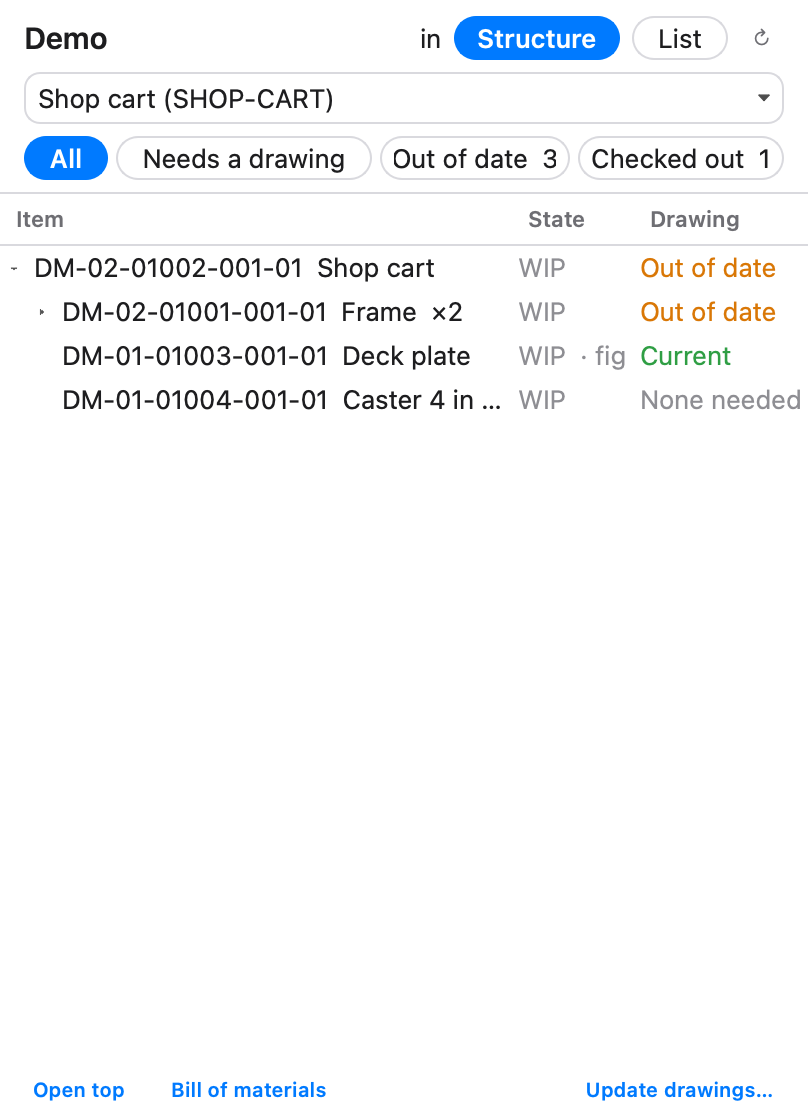
\includegraphics[width=0.46\linewidth]{fig/pdm09_structure_built.png}\hfill
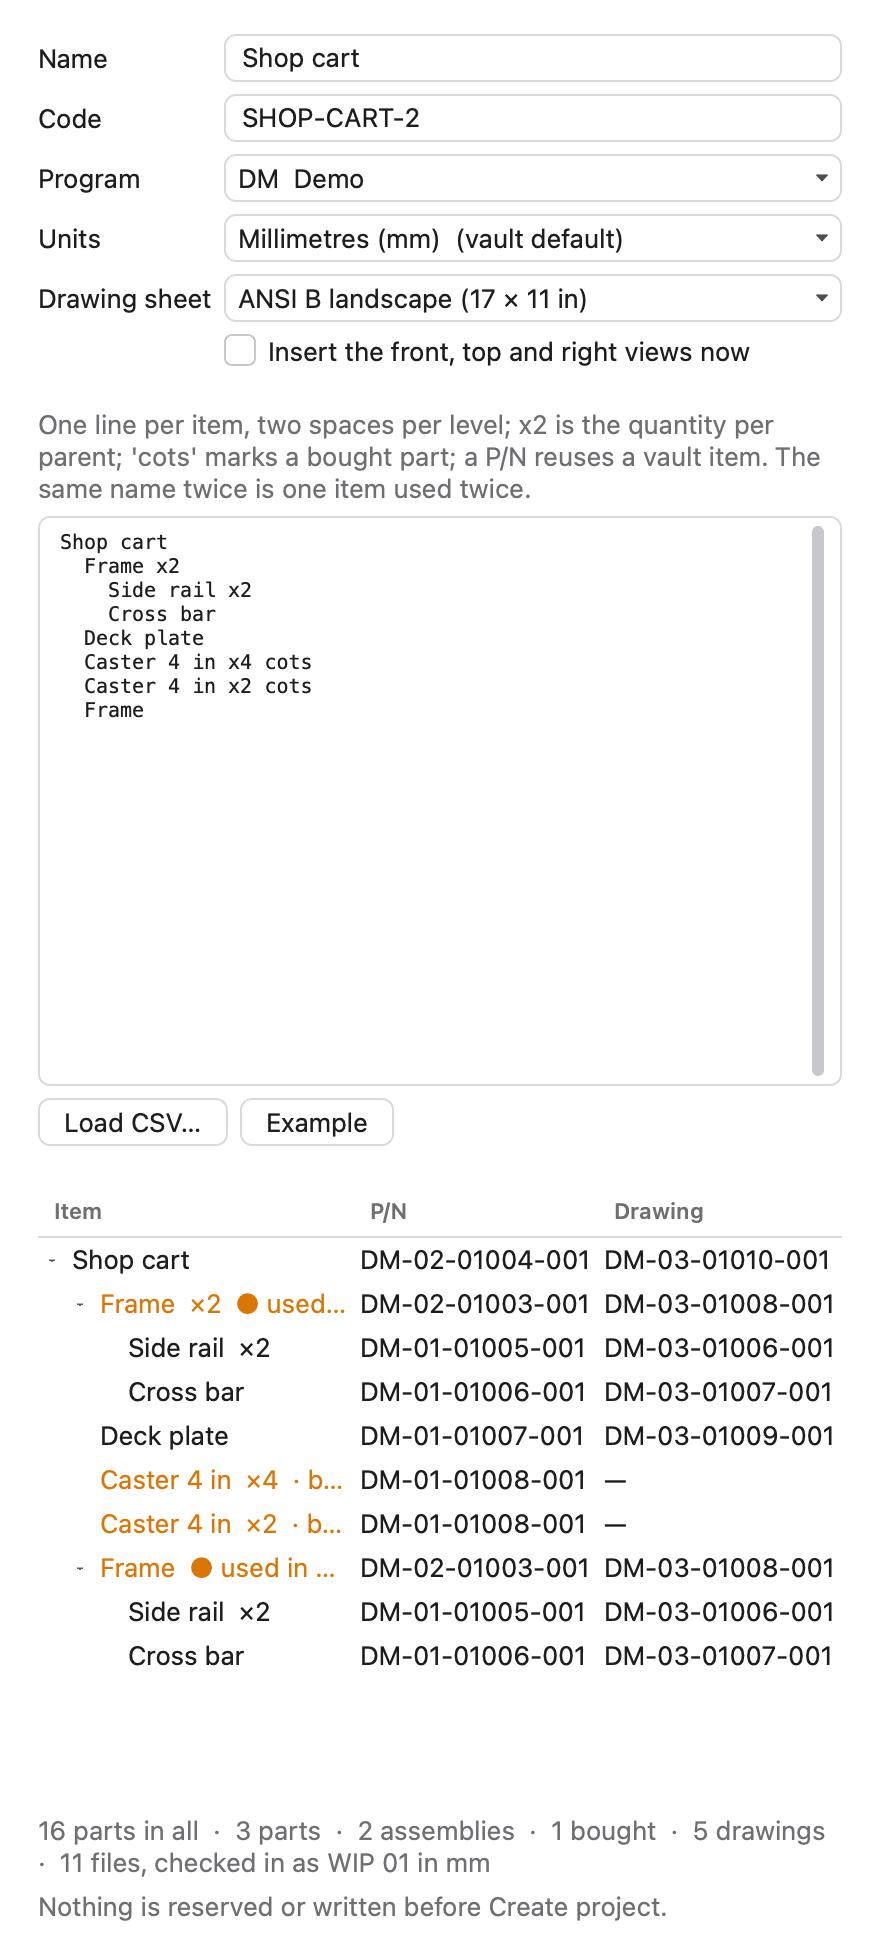
\includegraphics[width=0.50\linewidth]{fig/pdm09_wizard_built.png}
\caption{As built, rendered off screen. Left: the Vault tab's Structure view on a scratch project after the side
rail was modelled: the rail's, the frame's and the cart's drawings are out of date, the deck plate's is current,
the caster needs none; the chips carry the counts and the ``in'' badge says the project is in inches under a mm
vault. Right: the New Project panel's three boxes with a structure that names \emph{Frame} and \emph{Caster 4 in}
twice, so both carry the duplicate bubble; the preview shows every number and ``16 parts in all''.}
\label{fig:pdm09-built}
\end{figure}

\paragraph{Step 5 --- the Structure view} (\file{bruceworx\_structure.py}, the right panel's \code{BWVault} tab,
figure~\ref{fig:pdm09-built}). \emph{List | Structure} as two chips at the top, a root picker (the open projects
first, then every assembly) that follows an assembly selected in the Browser, the three filter chips with counts,
the tree with \emph{Item} (P/N-REV, description, $\times$quantity), \emph{State} (with ``from links'' and the
lock holder) and \emph{Drawing} coloured by state, lazy one level at a time (a placeholder row until the arrow is
clicked), the row menu (Open, Open drawing, Update drawing, Create drawing, Where used\ldots, Bill of materials\ldots,
Show in list, Show on the Start page) and the footer (Open top, Bill of materials, Update drawings\ldots, which
checks out each out-of-date drawing, opens it, recomputes it and opens the Check In panel for the first, listing
the rest). The empty state offers \emph{New Project\ldots}. It refreshes on every vault change through the vault
client's listener. \emph{Create drawing} makes a numbered blank drawing of an item that has none, checked in as
WIP~01 with \code{made\_from} over the item's closure.

\paragraph{Step 6 --- the engine} (\file{bruceworx/project\_setup.py}, 11 tests). The parser reads the plan's
text form (two spaces or a tab per level; \code{x2}, \code{2x} or \code{×2}; \code{cots}; a leading P/N reuses a
vault item; blank lines and \code{\#} comments skipped), a spreadsheet paste (tab-separated \emph{level, name,
qty, type}, header optional, levels relative) and CSV files (\emph{Load CSV\ldots}, \code{read\_structure\_file}),
into one rooted DAG: the same name is the same node, \code{uses} counts its parents, and the preview marks ``used in
$n$ places'' (answer~10). Errors: no root, two roots at the margin, a root without items, an item holding itself,
a bought part with children, a quantity below~1, a P/N as the top; a deeper indent than one level is read as one
level with a warning. \code{check} looks the reused P/Ns up (unknown, obsolete, a drawing), warns that items typed
under an existing item are not added to it, and refuses a retired program or document type. \code{plan\_numbers}
simulates the reservations on a copy of \file{numbering.json} (consecutive numbers, nothing written), flat, one
parent each; \code{order\_of\_work} is children first; \code{summary} gives $Q_t$ over the leaves as ``$N$ parts in
all'' with the counts of parts, assemblies, bought parts, reused items, drawings and files.

\paragraph{Step 7 --- the writer and the panel} (\file{bruceworx\_project.py}). \code{create\_project} does the
plan's steps 2--5 in order: files in \file{<vault>/.import/project-<id>}, children first (a part is an
\code{App::Part} with a Body and the vault's part properties, ``bought'' sets \code{ItemType}; an assembly is saved
\emph{before} its links, one \code{App::Link} per instance 50\,mm apart, the first child grounded with Assembly's
\code{GroundedJoint}; a drawing is its own file with a link to the model, saved before the link too, a blank page from
the template of the project's units and the title block filled, with \code{BWModel} naming its link so \emph{Insert
Views} can add the front, top and right views later); \emph{verify} reopens every staged assembly and compares the
walker's counts with the structure; then the numbers are taken, each file is numbered (P/N, revision~01, units,
and for a drawing the title block's part-number field) \emph{while its links still resolve}, renamed to
\file{<P/N>.FCStd} and relinked by name (\code{rewrite\_links}, \code{clear\_link\_errors}); then \code{create\_item}
for every item and drawing, \code{create\_project}, and one check-in per file: parts with their fingerprint
(\code{None} while empty), each assembly's BOM recorded for revision~01 from the structure as typed (so the
Structure view reads ``bom'', not ``from links''), drawings last with \code{made\_from} over their closure; work
copies fetched read-only; backups off throughout; staging removed. A failure before the numbers are taken leaves
the vault untouched (tested); after, the file is listed and its number stays unused, as an import does. The task
panel (figure~\ref{fig:pdm09-built}) has the project box (name, code made from the name, program, units with the
vault's default marked, drawing sheet following the units, the \emph{Insert views} tick box off by default), the
structure box (monospace text with the cart as placeholder, \emph{Load CSV\ldots}, \emph{Example}) and the preview
(item, P/N, drawing; the duplicate bubble in orange; the summary line; the issues in red), with \emph{Create
project} enabled only when the plan is complete; Create runs with a progress dialog, then opens the top and shows
the Structure view on the project. Entry points: \emph{File $\rightarrow$ New Project\ldots} (after New, put
back after every workbench change), the BruceWorx menu, the Start page's \emph{New Project\ldots} (its
\code{BruceWorx\_NewProject} hook now resolves), Cmd-K, and the Structure view's empty state. Headless:
\code{bw-hooks project preview --vault V --structure cart.txt} (numbers and issues, nothing written) and
\code{project new} (the same, then the files, inside \code{FreeCADCmd}; \code{--units}, \code{--sheet},
\code{--insert-views}, \code{--code}). Check-ins from the window now record the two fields through
\code{bruceworx\_vaultclient.CHECKIN\_EXTRAS}: a drawing's \code{made\_from} from the workspace, a part's fingerprint
from the open document (or the file, opened hidden); a failure there is logged and never stops the check-in.

\paragraph{Step 8 --- release and acceptance.} The release checklist has a sixth line, \emph{Drawing current (made
from this model)}, of a new kind \code{warn}: checked by the tool, orange with a ``!'' when the drawing was made from
an older version (metadata only passes; a pre-PDM-09 drawing is judged by time and says so), never a blocker and
recorded as \code{warning: true} with the approval (answer~6). Acceptance, headless in \code{FreeCADCmd}
(\file{TestBruceWorxProject.py}): the six-line cart on a scratch vault with inch standards becomes 6 items
(\code{DM-01}, \code{DM-02}) and 5 drawings (\code{DM-03}), every file WIP~01 with one version, \code{UnitSystem}
Imperial decimal in the top and in a drawing, the top's links by number with the walker counting 2 frames, 1 plate
and 4 casters, the first child grounded, the drawing blank with \code{BWModel} and the number in its title block,
every Drawing cell current and the caster ``none needed'', no staging or backup left; then the side rail gets a
$1\times1\times24$\,in box and is checked in with its fingerprint: the rail's, the frame's and the cart's drawings are
out of date (the frame's names the rail as the geometry change), the cross bar's and the plate's current, the top row
counts 2 below it, \emph{Update drawings} lists exactly those three; \emph{Insert Views} on the rail's drawing and a
check-in with \code{made\_from} make it current again while the frame's stays out of date; the checklist of the
frame warns and does not block. The same on a \textbf{copy of Vector} (\file{vector\_accept.py}, the CLI's
\code{project new} with \code{--units in} under program \code{LE}): \code{LE-02-01004-001} and ten more numbers
after the gearbox's, the project \code{SHOP-CART-ACCEPT} in inches under a mm vault, the same out-of-date chain
after the rail changed, Vector's own items untouched (``missing'': they have no drawing items). In the GUI:
\code{TestBruceWorxProject} (8), \code{TestBruceWorxChanges} (12), \code{TestBruceWorxVaultClient} (30) pass; the
hooks add-on's 300-odd stdlib tests pass.

\paragraph{Decided while building} (where the plan left a choice).
\begin{itemize}[nosep]
  \item \textbf{List is scoped to the root}, not the vault: every item under the picked project or assembly once,
        with its total quantity $Q_t$; vault browsing stays on the Start page (your 25 Oct decision). \emph{Show in
        list} selects the row there; \emph{Show on the Start page} finds it in the Files tree.
  \item \textbf{A project's code} is made from its name (\code{SHOP-CART}, unique with a numbered suffix) and can
        be edited; \code{update\_project} renames or closes it (closed projects leave the picker).
  \item \textbf{The project's units are recorded with it} (question~1, recommendation taken) and shown as the
        badge when they differ from the vault's; \code{drawing\_profile} is stored as the units until the
        drawing-standards profiles of step~2 give it another name.
  \item \textbf{The sheet}: inch projects on ANSI~B (question~4), mm projects on the vault's default sheet; the
        panel lets you pick another before Create.
  \item \textbf{Drawings are numbered as document type 03} (question~11) and their title block shows the
        drawing's number; the drawing-of link is the vault's. When PDM-07 settles the drawing key, the wizard
        changes one line.
  \item \textbf{A bought part is modelled too}: it gets a file (an empty part with \code{ItemType} cots) so the
        assembly can link it; it gets no drawing. A reused P/N is linked from its work copy and typed items under it
        are not added to it (its structure is its own file's).
  \item \textbf{Each assembly's BOM is recorded at creation} from the structure as typed, with the version it
        describes, so the Structure view and where-used are exact from the first minute; a later check-in's walker
        replaces it as usual.
  \item \textbf{An empty part has no fingerprint}, so a change to it before it has a shape counts as geometry
        (there is nothing to compare); the first modelled version starts the fingerprints.
  \item \textbf{The assembly drawing's closure uses the recorded BOM, else the file's links} (question~9), both in
        the Structure view and in the checklist line, so an older vault without BOMs still gets the chain.
  \item \textbf{Instances in a row, 50\,mm apart}, the first grounded: enough for empty parts to open without
        overlapping; the user places them when modelling.
  \item \textbf{The Insert Views command} lives on the drawing (\code{BruceWorx\_InsertViews}, active when the
        document's page names its model); the panel's tick box inserts them at creation instead (answer~8).
\end{itemize}

\paragraph{Questions after steps 4--8.}
\begin{enumerate}[nosep]
  \item \textbf{Projects on the Start page.} The dashboard lists recorded projects by code and name now; should
        the Start page's project row open the Structure view on it (one call), and should \emph{New Project} be
        offered beside \emph{New Part} in the toolbar? \emph{Recommendation:} yes to both.
  \item \textbf{Update drawings and several files.} It opens the Check In panel for the first drawing and lists
        the rest (one panel at a time). Should it instead check them all in at once with one comment, as the
        check-in panel's rows do? \emph{Recommendation:} yes, once you have seen the recomputed sheets once.
  \item \textbf{Out of date through metadata of an assembly.} An assembly's own file changes with every placement
        or link edit and has no fingerprint, so its drawing reads ``out of date'' after any save of the assembly.
        Fingerprint assemblies too (the compound of their instances)? \emph{Recommendation:} yes, in a later pass,
        with the same seven digits.
  \item \textbf{Family numbers.} The wizard numbers flat (one parent each); the spike showed family numbers collide
        across document types. Keep flat until Ops allocates? \emph{Recommendation:} keep flat.
\end{enumerate}
